\section{A*}\label{sec:a_star}

%Přesný popis A* algoritmu.

\nameref{sec:a_star} je známý prohledávací algoritmus pro~rychlé hledání nejkratších cest.
Algoritmus potřebuje znát prohledávací prostor určený možnými stavy.
Dále je nutné uvést určitou \emph{heuristiku}, která pro~určitý vrchol vrátí
spodní odhad na~cenu zbylé cesty z~aktuálního stavu do~cílového stavu.
Algoritmus si zároveň pamatuje pro~každý navštívený stav cenu cesty z~počátečního stavu do~aktuálního.
\nameref{sec:a_star} postupně prochází frontu navštívených stavů.
Při~procházení odebere stav z~fronty a poté pro~daný stav přidá sousední stavy do~fronty.
Vybraný stav z~fronty je určen nejmenším součtem cenou cesty
do~aktuálního stavu z~počátečního a heuristiky v~aktuálním stavu.
Tento součet je spodní odhad na~minimální cenu cesty z~počátku do~cíle vedoucí přes navštívené stavy,
přes~které byl aktuální vrchol dosažen.
\nameref{sec:a_star} zaručuje při~tomto postupu optimalitu nalezené cesty.

V~následujících kapitolách popíšu dvě různé implementace \nameref{sec:a_star} algoritmu pro~řešení problému křižovatky.

\subsection{Individuální A* (\ref{str:a_star_ars})}\label{subsec:individualni_a_star}\labeltext{A*RS}{str:a_star_ars}

%Popis úpravy A* algoritmu pro řešený problém, parametry a pseudokód.

\ref{str:a_star_ars} patří do~kategorie \ref{str:rs} algoritmů.
Plánuje stejně jako \nameref{sec:safe_lanes}, jednoho agenta po~druhém.
Akorát tentokrát algoritmus dovoluje agentům \uv{opustit} svoje~pruhy.

Pro~správné fungování \nameref{sec:a_star} je potřeba vhodně vybrat cenu cesty a heuristiku.
Cena cesty se počítá podobně jako při~hledání \hyperref[par:pruh]{pruhu} v~křižovatce.
Cena je složena z více kritérií, a to \hyperref[par:ars_vzdalenost]{vzdálenost},
\hyperref[par:ars_uhel_zataceni]{úhel zatáčení} a \hyperref[par:ars_pocet_zataceni]{počet zatáčení}.
Priorita kritérií je nejprve podle menší \hyperref[par:ars_vzdalenost]{vzdálenosti},
poté menšího \hyperref[par:ars_uhel_zataceni]{úhlu zatáčení}
a nakonec vyššího \hyperref[par:ars_pocet_zataceni]{počtu zatáček}.
Takto jsem se rozhodl, protože chci najít nejkratší cesty do~cíle.
Pokud existuje více stejně dlouhých cest do~cíle, chci vybrat nejvíce \uv{příjemnou} cestu pro~pasažéry auta.
Pokud má více cest všechny kritéria stejné, mají všechny stejnou cenu.

\paragraph{Vzdálenost}\label{par:ars_vzdalenost} je počet hran grafu, přes~které cesta vede.
Duplicitní hrany se započítávají vícekrát.
Pokud agent stojí na místě, vzdálenost se nemění.

\paragraph{Úhel zatáčení}\label{par:ars_uhel_zataceni} určuje úhel, o~který se musí agent při~sledování cesty otočit.
Pro~každý prostřední vrchol se na~cestě dopočítá úhel mezi hranami,
přes~kterou se agent na~vrchol dostal a kterou odjel.
Tento úhel se dá jednoduše geometricky dopočítat, jelikož známe přesnou pozici vrcholů.
\nameref{par:ars_uhel_zataceni} je součet absolutních hodnot těchto úhlů.

\paragraph{Počet zatáčení}\label{par:ars_pocet_zataceni} udává počet
nenulových \hyperref[par:ars_uhel_zataceni]{úhlů zatáčení}.

\paragraph{Heuristika}\label{par:ars_heuristika} v tomto případě je minimální počet hran cesty
z~aktuálního vrcholu do~nejbližšího z~cílových vrcholů.
Při~tomto výpočtu ignoruji všechny agenty na~křižovatce.
Pokud žádná taková cesta neexistuje, je hodnota \hyperref[par:ars_heuristika]{heuristiky} $\infty$.

Heuristika nebere v~úvahu úhel ani počet zatáčení.
Tato \hyperref[par:ars_heuristika]{heuristika} je přípustná, dokonce i~monotónní.

Prohledávací prostor jsou vrcholy křižovatky rozšířené o~krok, ve~kterém by agent na~daný vrchol přijel.
Následující stavy daného stavu jsou všechny validní stavy dané sousedy vrcholu aktuálního stavu.
Formálně pro~vrchol $u$ jsou jeho sousedi vrcholy $\{v \in V | (u,v)\in E\}$,
kde $V$ je množina vrcholů a $E$ je množina hran.

\subsubsection{Parametry}\label{subsubsec:ars_parametry}
Pro~reálnější pohyby agentů po~křižovatce je vhodné omezit množinu sousedů vrcholu.
Avšak určení vhodného omezení je komplikované.
Proto jsem se rozhodl umožnit omezení měnit parametry.
Zároveň parametry napomáhají rychlejšímu prohledávání omezením prohledávaného prostoru.
Bohužel při~nastavení parametrů algoritmus ztrácí svojí optimalitu.

\paragraph{Maximum návštěv vrcholu (\ref{par:ars_mnv})}\labeltext{MNV}{par:ars_mnv}
udává maximální počet výskytů libovolného vrcholu na~cestě.
Proto jsou validní hodnoty kladná celá čísla.
Nejreálnější hodnota parametru by byla $1$, není pro~auto moc přirozené jezdit ve~smyčkách.
Avšak vyšší hodnoty mohou vést k~obecně lepšímu řešení.
Na obrázku (Obrázek \ref{fig:ars_mnv_example}) je vyobrazen příklad takové situace.
Agent $a$ cestuje z $A$ do $B$, agent $b$ cestuje z $B$ do $C$.
Pokud by agenti mohli navštívit každý vrchol nejvýše jednou, neexistují nekolizní trasy pro~oba agenty najednou.
Avšak pokud povolíme alespoň dvě návštěvy vrcholu, existuje pro~agenta $a$ trasa $A, 1, 2, 1, 2, 3, 4, B$
a pro~agenta $b$ cesta $C, 4, 3, 2, 5, D$.

\begin{figure}[h]
	\centering
	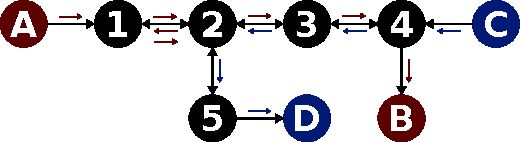
\includegraphics[width=140mm]{../img/mnv_example}
	\caption{Situace, při které neexistují cesty pro~oba agenty, aniž by se aspoň jeden vracel na navštívený vrchol}
	\label{fig:ars_mnv_example}
\end{figure}

\paragraph{Povolené zastavování (\ref{par:ars_pz})}\labeltext{PZ}{par:ars_pz}
určuje, zda-li může agent stát na~místě.
Formálněji pokud dovolím zastavování, vrchol se stane sám sobě sousedem a může se vyskytovat vícekrát na~cestě za~sebou.
Jednotlivé stání na~místě se pořád započítávají jako jednotlivé návštěvy,
tudíž maximální doma stání musí být menší než~hodnota \ref{par:ars_mnv}.

\paragraph{Maximální prodleva při~cestě (\ref{par:ars_mpc})}\labeltext{MPC}{par:ars_mpc}
omezuje počet kroků strávených agentem na~křižovatce.
Nalezená trasa pro daného agenta musí trvat nejvýše $\ref{par:ars_mpc} + p$ kroků,
kde $p$ je počet kroku optimální cesty (doba jízdy v~\hyperref[par:pruh]{pruhu}).
Hodnota $0$ znamená, že agent může jet pouze cestou stejného počtu kroků
jako je počet kroků jízdy v \hyperref[par:pruh]{pruhu}.
Tento parametr slouží jako omezení hloubky prohledávání.

\paragraph{Povolené vracení (\ref{par:ars_pv})}\labeltext{PV}{par:ars_pv}
může agentovi zakázat vracet~se na~vrchol, ze~kterého přijel.
Tento parametr dovoluje agentovi pouze \uv{jízdu dopředu}, což je přirozené od~jízdy v~autě očekávat.
Formálně pokud je tento parametr nenastaven, jsou zakázány cesty obsahující $u,v,v,\dots,v,u$,
kde $u, v \in V$ a $u \neq v$.
Posloupnost vrcholů $v$ musí být dlouhá alespoň jedna, avšak není zhora omezená.

\subsubsection{Sousední stavy}\label{subsubsec:sousedni_stavy}

Nyní blíže popíšu výběr následujícího stavu.
Přesněji popíšu funkci \ref{subsubsec:sousedni_stavy}\labeltext{\textrm{neighbour\_states}}{alg:sousedni_stavy},
která dostává na~vstup stav a vrací následující množinu platných stavů.
Množina následných stavů je ovlivněna \hyperref[subsubsec:ars_parametry]{parametry}.
Avšak většinou se jedná o~podmnožinu sousedních vrcholů aktuálního vrcholu, popřípadě ještě aktuální vrchol.
Tuto~množinu budu nazývat \emph{sousedi}\labeltext{sousedi}{str:ars_sousedi}.

Pro~získání \hyperref[str:ars_sousedi]{sousedů} začnu s~množinou všech vrcholů,
do~kterých vede hrana z~vrcholu aktuálního stavu.
Budu předpokládat, že tuto množinu je jednoduše možné získat z~grafu křižovatky.
Pokud je nastavený \hyperref[subsubsec:ars_parametry]{parametr} \ref{par:ars_pz},
přidám do~množiny \hyperref[str:ars_sousedi]{sousedů} aktuální vrchol.

Agent se nesmí srazit s~žádným jiným naplánovaným agentem při~jízdě do~sousedního vrcholu.
Kolizní přejezdy jsou detekovány způsobem popsaným v~sekci \nameref{sec:kolize}.

Pro~kontrolu \hyperref[subsubsec:ars_parametry]{parametru} \ref{par:ars_mnv}
je možné projít všechny předchozí stavy až po~počáteční
a odebrat všechny vrcholy vyskytující se alespoň \ref{par:ars_mnv} krát během tohoto průchodu.
Následující pseudokód zobrazuje přesnější postup odstraňování.

\labeltext{\textrm{control\_MNV}}{alg:ars_mnv}
% @formatter:off
\begin{code}[fontsize=\footnotesize]
// MNV předem nastavená hodnota maxima návštěv vrcholu

// vstup aktuální stav, množina sousedních vrcholů
// výstup množina sousedů navštívená nejvýše MNV - 1
control_MNV(state, neighbours)
  occurs <- empty // slovník návštěv vrcholů s implicitní hodnotou 0
  predecessor <- state
  while predecessor is not NULL
    occurs[predecessor.vertex] <- occurs[predecessor.vertex] + 1
    predecessor <- predecessor.parent
  for vertex in neighbours
    if occurs[vertex] >= MNV
      neighbours.remove(vertex)
  return neighbours
\end{code}
% @formatter:on

Pokud je hodnota \hyperref[subsubsec:ars_parametry]{parametru} \ref{par:ars_mpc} konečná,
je možné provést filtrování sousedních vrcholů podle nejkratší vzdálenosti ze~souseda do~nejbližšího cíle.
Tuto vzdálenost vím díky heuristice, která má stejnou hodnotu.
Nejprve si spočítám maximální krok cesty\labeltext{MKC}{str:ars_mkc} (\ref{str:ars_mkc}) pro~daného agenta.
Pokud sečtu aktuální plánovaný krok s~hodnotou heuristiky počátečního vrcholu, dostanu nejmenší krok,
ve~kterém se může agent dostat do~nejbližšího cíle.
\ref{str:ars_mkc} přiřadím součet této hodnoty a \ref{MPC}.
Jednoduše je vidět, že agent nemůže dorazit do~cíle po~kroku \ref{str:ars_mkc},
aniž~by porušil podmínku určenou parametrem \ref{alg:ars_mpc}.

Následně mohu zkontrolovat, jestli se agent může dostat ze~sousedního vrcholu
do~některého cíle do~kroku \ref{str:ars_mkc}.
Vzdálenost souseda do~nejbližšího cíle zjistím z~heuristiky.
Tudíž stačí porovnat součet kroku stavu a heuristiky souseda s~hodnotou \ref{str:ars_mkc}.
Přesný vzhled filtrace je popsán v následujícím pseudokódu.

\labeltext{\textrm{control\_MPC}}{alg:ars_mpc}
% @formatter:off
\begin{code}[fontsize=\footnotesize]
// MKC předem spočtená hodnota maximálního kroku cesty
// heuristics množina vzdáleností do nejbližšího cíle indexovaná vrcholy

// vstup aktuální stav, množina sousedních vrcholů
// výstup množina sousedů dostatečně blízkých cílům
control_MPC(state, neighbours):
  for vertex in neighbours
    if state.step + heuristics[vertex] >= MKC:
      neighbours.remove(vertex)
  return neighbours
\end{code}
% @formatter:on

Poslední filtrování sousedů probíhá pouze, pokud je nastaven
\hyperref[subsubsec:ars_parametry]{parametr} \ref{par:ars_pv}.
Opět lze při~kontrole využít procházení předchozích stavů.
Přesněji nejprve naleznu nejpozději navštívený vrchol před~aktuálním.
Pokud takový vrchol neexistuje, mohu skončit.
Jinak odeberu tento vrchol ze~sousedů.
Následující pseudokód zobrazuje přesnější průběh.

\labeltext{\textrm{control\_PV}}{alg:ars_pv}
% @formatter:off
\begin{code}[fontsize=\footnotesize]
// PV předem nastavená hodnota parametru povolení vrácení

// vstup aktuální stav, množina sousedních vrcholů
// výstup množina sousedů s odebraným předchozím vrcholem
control_PV(state, neighbours)
  if PV
    return neighbours
  predecessor <- state.parent
  while predecessor is not NULL and predecessor.vertex is state.vertex
    predecessor <- predecessor.parent
  if predecessor is not NULL
    neighbours.remove(predecessor.vertex)
  return neighbours
\end{code}
% @formatter:on

Nyní již můžu definovat funkci \ref{alg:sousedni_stavy} jako funkci, která vygeneruje validní sousední stavy.
Funkce nejprve pomocí funkce \textrm{neighbours} vygeneruje sousední vrcholy.
Poté~odstraní neplatné sousedy funkcemi \textrm{collision\_free},
\ref{alg:ars_mnv}, \ref{alg:ars_mpc} a \ref{alg:ars_pv}.
Nakonec pro~každý zbylý vrchol vytvoří nový stav.

Pro~vytvoření následujícího stavu je potřeba znát
úhel mezi vrcholy předchozího stavu, aktuálního stavu a dotyčného sousedního vrcholu.
Přesný výpočet zde vynechám.
Budu předpokládat, že se mohu zeptat grafu křižovatky na~tento úhel.

Pseudokód celkové funkce na~generování sousedních stavů je níže.


% @formatter:off
\begin{code}[fontsize=\footnotesize]
// G graf křižovatky
// funkce angle(u, v, w) na výpočet úhlu mezi třemi vrcholy
// heuristics množina vzdáleností do nejbližšího cíle indexovaná vrcholy

// vstup aktuální stav, poloměr agenta
// výstup množina sousedních stavů
neighbour_states(state, da)
  neighbours <- neighbours(state)
  neighbours <- collision_free(state, neighbours, da)
  neighbours <- control_MNV(state, neighbours)
  neighbours <- control_MPC(state, neighbours)
  neighbours <- control_PV(state, neighbours)

  current_vertex <- state.vertex
  last_vertex <- NULL
  if state.parent is not NULL
    last_vertex <- state.parent.vertex
  states <- empty

  for vertex in neighbours
    neighbour_state <- new
    neighbour_state.step <- state.step + 1
    if current_vertex is vertex
      neighbour_state.distance <- state.distance
    else
      neighbour_state.distance <- state.distance + 1

    angle <- 0
    if last_vertex is not NULL
      angle <- angle(last_vertex, current_vertex, vertex)
    neighbour_state.angle <- state.angle + angle
    if angle is 0
      neighbour_state.turns <- state.turns
    else
      neighbour_state.turns <- state.turns + 1
    neighbour_state.heuristics <- heuristics[vertex]
    states.add(neighbour_state)

  return states
\end{code}
% @formatter:on

\subsubsection{Výsledný algoritmus}\label{subsubsec:ars_vysledny_algoritmus}

Nakonec popíšu kompletní upravený \nameref{subsec:individualni_a_star} algoritmus.

Pro~zrychlení prohledávání použiji \emph{graph-search} variantu \nameref{sec:a_star} algoritmu.
V~této variantě si algoritmus pamatuje navštívené stavy (stavy odebrané z~fronty).
Z~množiny sousedních stavů je možné odebrat všechny navštívené stavy.
U tohoto algoritmu jsou stavy totožné, pokud mají stejný vrchol, stejný krok a zároveň vrcholy všech předků si odpovídají.
Nutnost shody všech předků vyplývá z použití dodatečných parametrů, které omezují množinu sousedů.
Například pokud se dostanu na stejný vrchol ve stejný krok ze dvou různých vrcholů
a povolím pouze jedno navštívení vrcholu, sousední stavy se u obou variant budou lišit.

Během testování jsem zjistil, že kontrola pouze rovnosti posledního vrcholu a předchozího stavu
značně zrychluje běh algoritmu, aniž by~se výrazně zhoršilo plánování.
Proto jsem se rozhodl udělat kompromis a určit, že dva stavy jsou si rovné právě tehdy,
když mají stejný vrchol, krok, a jejich rodiče mají stejný vrchol.

Nejprve je nutné pro~daného agenta spočítat heuristiku pro~každý vrchol.
To mohu provést procházením přes~cílové vrcholy.
Pro~každý cíl spočtu vzdálenost od~každého vrcholu do~tohoto cíle.
Pokud je tato hodnota menší než zatím nejmenší nalezená vzdálenost, přepíši tuto hodnotu.
Pro~účely počítání vzdálenosti mezi vrcholy si můžu tyto vzdálenosti uložit předem ke~grafu.
Tyto hodnoty lze získat například Floyd–Warshallovým algoritmem (\citet*{Floyd-Warshall}).
Poté se spočte hodnota posledního kroku \ref{str:ars_mkc} a uloží se pro~pozdější použití.

Následně algoritmus vygeneruje počáteční stav a přidá ho do~fronty prohledávaných stavů.
Poté~algoritmus odebere z~fronty nejmenší stav podle součtu ceny cesty do~vrcholu stavu a heuristiky.
Pokud vrchol odebraného stavu je mezi cílovými, zkonstruuje se cesta a přiřadí se agentovi.
Plánování agenta je v~tomto případě hotové, už~zbývá jen přidat naplánovanou cestu
do~\hyperref[par:obsazene_pozice]{tabulky obsazených pozic}, aby nedošlo ke~kolizi s~pozdějšími agenty.
Agent je následně vrácen zpět \hyperref[sec:simulace]{simulátoru}.

Pokud vrchol stavu není mezi cílovými,
získají se pomocí výše popsaného postupu sousední stavy a přidají se do~fronty.
Takto algoritmus pokračuje, dokud nenalezne validní cestu, nebo není fronta prázdná.
V~tom případě nemůže být agent naplánován, jeho cestování je pozdržené, a simulátoru se vrátí $NULL$.

Konstrukci cesty provedu postupným procházením předků koncového stavu.
Pro~každý takový stav přidám na~začátek cesty vrchol zmíněného stavu.
Tento postup budu opakovat, dokud nenarazím na předka s rodičem $NULL$.
Tento postup nazvu \ref{alg:ars_construct_path}\labeltext{\textrm{construct\_path}}{alg:ars_construct_path}.

% @formatter:off
\begin{code}[fontsize=\footnotesize]
// vstup finální stav cesty
// výstup kompletní cesta z vrcholů
construct_path(state)
  path <- empty
  while state is not NULL
    path.addFirst(state.vertex)
    state <- state.parent
\end{code}
% @formatter:on


Následující pseudokód zachycuje celý \nameref{subsec:individualni_a_star} algoritmus.

% @formatter:off
\begin{code}[fontsize=\footnotesize]
// G graf křižovatky se vzdálenostmi mezi vrcholy
// MPC parametr maximální prodlevy cesty

// vstup krok, plánovaný agent
// výstup agent nebo NULL
plan_agent(step, agent)
  MKC <- step + MPC + heuristics[entry]
  da <- agent.diameter

  // prioritní fronta porovnávající prvky podle součtu ceny cesty a heuristiky
  queue <- emptyPriorityQueue
  initial_state <- empty
  initial_state.vertex <- agent.entry
  initial_state.step <- agent.step
  initial_state.heuristics <- heuristics[entry]
  queue.push(initial_state)

  while not queue.empty()
    state <- queue.pop()
    if agent.exits.contain(state.vertex)
      agent.path <- construct_path(state)
      add_planned_agent(step, agent)  // přidání agenta do obsazených pozic
      return agent
    else
      queue.addAll(neighbour_states(state, da))

  return NULL
\end{code}
% @formatter:on


\subsection{Hromadný A*}\label{subsec:hromadny_a_star}

Rozšíření A* pro více agentů, popis vylepšení.
Parametry, pseudokód.

\subsection{Conflict-Based Search (\ref{str:cbs})}\label{subsec:conflict_based_search}\labeltext{CBS}{str:cbs}

%Popis algoritmu, úprava pro můj problém.
%Parametry, pseudokód.

\nameref{subsec:conflict_based_search} algoritmus \citep*{Sharon} rozšiřuje jakýkoliv \ref{str:rs} algoritmus
na multiagentní plánování.
V mém případě budu rozšiřovat \ref{str:a_star_ars}.

\ref{str:cbs} začíná individuálním naplánováním všech agentů nezávisle na~sobě.
Čili agenti nesmějí mít kolize s~již cestujícími agenty,
avšak mohou mí kolizní trajektorii s~jinými aktuálně plánovanými agenty.
Poté se zkontroluje, zda-li nemají nějací agenti kolizní trajektorie.
Pokud ne, plánování úspěšně končí.
Jinak se prohledávání rozdělí na dva případy.
V obou případech je přeplánován jeden agent s podmínkou, že se musí vyhnout koliznímu místu.
Poté se opakuje opětovné hledání kolizí a rozdělování na případy.
Aby nedošlo k zacyklení, je nutné při plánování agenta vyhnout se nejen aktuální kolizi, ale také všem předchozím.
Výpočet postupně vytváří strom,
kde každý vrchol obsahuje cesty agentů (mohou být navzájem kolizní) a tabulku zakázaných pozic.
Algoritmus skončí v~prvním nalezeném vrcholu neobsahujícím kolizní trasy.

Již cestující agenti mohou omezovat trasy natolik, že pro agenta neexistuje žádná nekolizní cesta skrze křižovatku.
Dále se může stát, že agent nenajde žádnou nekolizní cestu, která by nevedla místo, které bylo dříve označené jako kolizní.
V obou případech plánování tohoto agenta selže a agent zcela odstraněn z~vrcholu.
Následně jsou nalezeni agenti, kteří byli v~historii přeplánováni kvůli odstraněnému agentovi.
Pro~tyto agenty jsou nalezeny nové cesty, jelikož pro~ně může existovat lepší cesta.

Algoritmus postupně prochází listy stromu výpočtu.
Pořadí průchodu je určeno počtem agentů.
Pokud je počet agentů u~více listů shodný, vybere se vrchol s nejmenší vzdáleností podobně jako u \ref{str:a_star_arsg}.
Algoritmus naplánuje pouze agenty, kteří mají cesty ve~vybraném listu, vjezd zbylých agentů je zamítnut.

\ref{str:cbs} najde optimální cestu pro všechny agenty \citep{Sharon}.
Avšak velikost stromu může být obrovská.
Proto jsem se rozhodl obětovat optimalitu a zjednodušit práci algoritmu, pokud plánování trvá příliš dlouhou dobu.
Ve zjednodušeném režimu algoritmus přeplánuje takovým způsobem, aby neměl žádné kolize s ostatními plánovanými agenty.
To znamená, že v tomto režimu plánuje algoritmus agenty stejně jako \ref{str:a_star_ars}.


\subsubsection{Parametry}\label{subsubsec:cbs_parametry}

\nameref{subsubsec:cbs_parametry} algoritmu jsou stejné jako u \ref{str:varsg} a mají podobný význam.
Hodnoty Maximum návštěv vrcholu (\ref{str:ars_mnv}), Povolené zastavování (\ref{str:ars_pz}),
Maximální prodleva při~cestě (\ref{str:ars_mpc}) a Povolené vracení (\ref{str:ars_pv})
algoritmus používá při~plánování jednoho agenta.
Tyto \hyperref[subsubsec:ars_parametry]{parametry} ovlivňují plánování stejně jako u \ref{str:a_star_ars}.
Hodnota parametru \ref{str:arsg_zvp} opět určuje po jak dlouhé prodlevě má algoritmus přejít na zjednodušené plánování.

\subsection{CBS-OID}\label{subsec:cbsoid}

\ref{str:cbs} lze podobně jako \ref{str:varsg} rozšířit na \ref{str:suboid} variantu.
K plánovaným agentů se přidají agenti z předchozích kroků.
Jako počáteční cesty těchto agentů se použijí jejich již naplánované trasy, tudíž se znova nepočítají.
Výpočet je poté shodný, až na~případy, kdy pro~ně nebyla nalezena cesta.
Pokud k~takové situaci dojde, namísto odstranění agenta se odstraní celý list ze~stromu výpočtu.

Parametry jsou rozšířené stejně jako u \nameref{subsubsec:a_star_aoid} o~Maximální počet agentů (\ref{str:aoid_mpa})
a Počet přeplánovaných kroků (\ref{str:aoid_ppk}).
Význam těchto parametrů je shodný.

